Im nachfolgenden Abschnitt werden mögliche Wege zweier Angriffsziele aufgezeigt, die Personen bei jugendliche Nutzer anwenden können. Zunächst wird ein Graph eingeführt, der diese Angriffsszenarien verbildlicht. Danach wird die Umsetzung dieser Schritte mit den jeweiligen Apps erklärt.


\begin{figure}[h!]
\centering
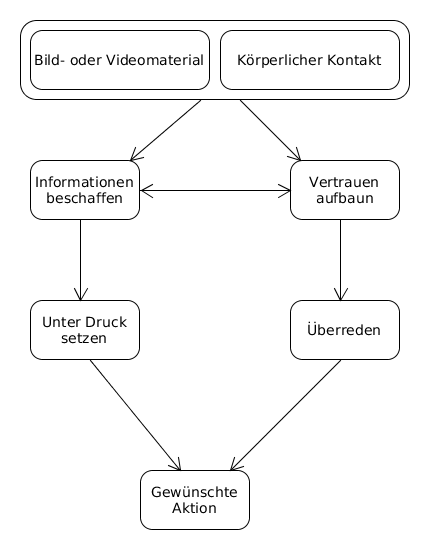
\includegraphics[width=0.5\textwidth]{./resources/angriffsvektoren}
\caption{Einfache Angriffswege}
\label{vektoren_overview}
\end{figure} 



In Abbildung \ref{vektoren_overview} werden zwei mögliche Ziele und deren Umsetzungsschritte vereinfacht verbildlicht. Dabei werden nicht alle möglichen Schritte und deren Kombinationen abgehandelt. Das Schaubild soll lediglich zwei einfache Szenarien behandeln, um jeweils zwei mögliche Ziele zu erreichen. Als erstes Ziel wird die Beschaffung von Bild- oder Videomaterial von der jugendliche Person definiert.
Das zweite Ziel ist der körperliche Kontakt, der eine Person zu der oder dem Jugendlichen erreichen möchte. 

\subsection{Informationen beschaffen um damit Druck auszuüben.}

Die Idee bei diesem Weg ist, so viel Informationen zu beschaffen, mit dem der oder die Jugendliche unter Druck gesetzt werden kann. Ein Druckmittel könnte ein Geheimnis von den Eltern oder unangenehme Informationen von den Jugendlichen sein, die nicht veröffentlicht werden sollten. Mit diesen Druckmittel kann dann das Opfer für Handlungen gezwungen werden.

\paragraph{Bei YouNow}kann jeder, auch ohne eine Anmeldung die Videos von Jugendlichen ansehen, ohne dass die betreffende Person etwas davon mitbekommt. Hier wäre es möglich über einen längeren Zeitraum belastende  Informationen zu suchen. Denkbar wäre auch gezielte Fragen zu stellen, mit denen man weitere Schritte unternehmen könnte. Dazu müsste man sich allerdings anmelden. 

\paragraph{Bei Snapchat} ...

\subsection{Vertrauen aufbauen um die betreffende Person zu überreden.}
Für diesen Schritt muss sich der Jugendliche über einen gewissen Zeitraum auf die Person einlassen. Denkbar wäre im Vorfeld eine Informationsbeschaffung um gezielter zu manipulieren oder das Vertrauen für die Informationsbeschaffung zu nutzen. 

\paragraph{Bei YouNow}, wie bei allen anderen Internetdiensten, ist es nicht möglich sicherzustellen, dass sich hinter einer Person auch diese verbirgt. Man kann ohne weiteres sich einen Account erstellen.  Für die Kontaktaufnahme ist der Chat neben dem Stream zur verfügung. Außerdem gibt es noch die Möglichkeit dem Jugendlichen persönlich zu schreiben. 

\paragraph{Bei Snapchat} ...